\documentclass[11pt]{article}

\usepackage{geometry, amsmath, amsthm, latexsym, amssymb, graphicx, caption, float, graphbox}
\geometry{margin=1in, headsep=0.25in}

\captionsetup[figure]{labelfont={bf},name={Fig.}}

\parindent 0in
\parskip 0pt

\begin{document}

\title{cs229-milestone}

\thispagestyle{empty}

\begin{center}
{\large \bf Identifying Transcription Unit Structure from Rend Sequencing Data} \\
Category: Life Sciences \\
Travis Horst (thorst)
\end{center}

\textbf{Motivation} \vspace{4pt} \\
In bacteria, many genes are expressed together on the same RNA transcript called a transcription unit (TU).  Identifying these TUs can play a role in better understanding biology as related genes are typically expressed together and coexpression can have important physiological implications.  Although many TUs have been identified, there is not an efficient way to determine all the TUs.  Sequencing techniques can provide high throughput data of the transcripts in populations of bacteria.  Recent work (Fig. \ref{fig:lalanne_reads}),\textsuperscript{1} has shown promise in identifying TUs however the analysis (peak z-score) was not generally applicable to entire genomes.  Analysis of this data across the entire genome would allow progress to be made in improving models of whole cells.\textsuperscript{2}  Rend seq data, as provided in the work by Lalanne,\textsuperscript{1} can provide benefits over other sequencing data as it does not suffer from 3' end bias and shows enrichment at the start and end of TUs as seen by spikes in the read count plots.  This makes the data an ideal candidate for applying unsupervised machine learning techniques to uncover the TU structure contained in the read data.

\begin{figure}[H]
    \centering
    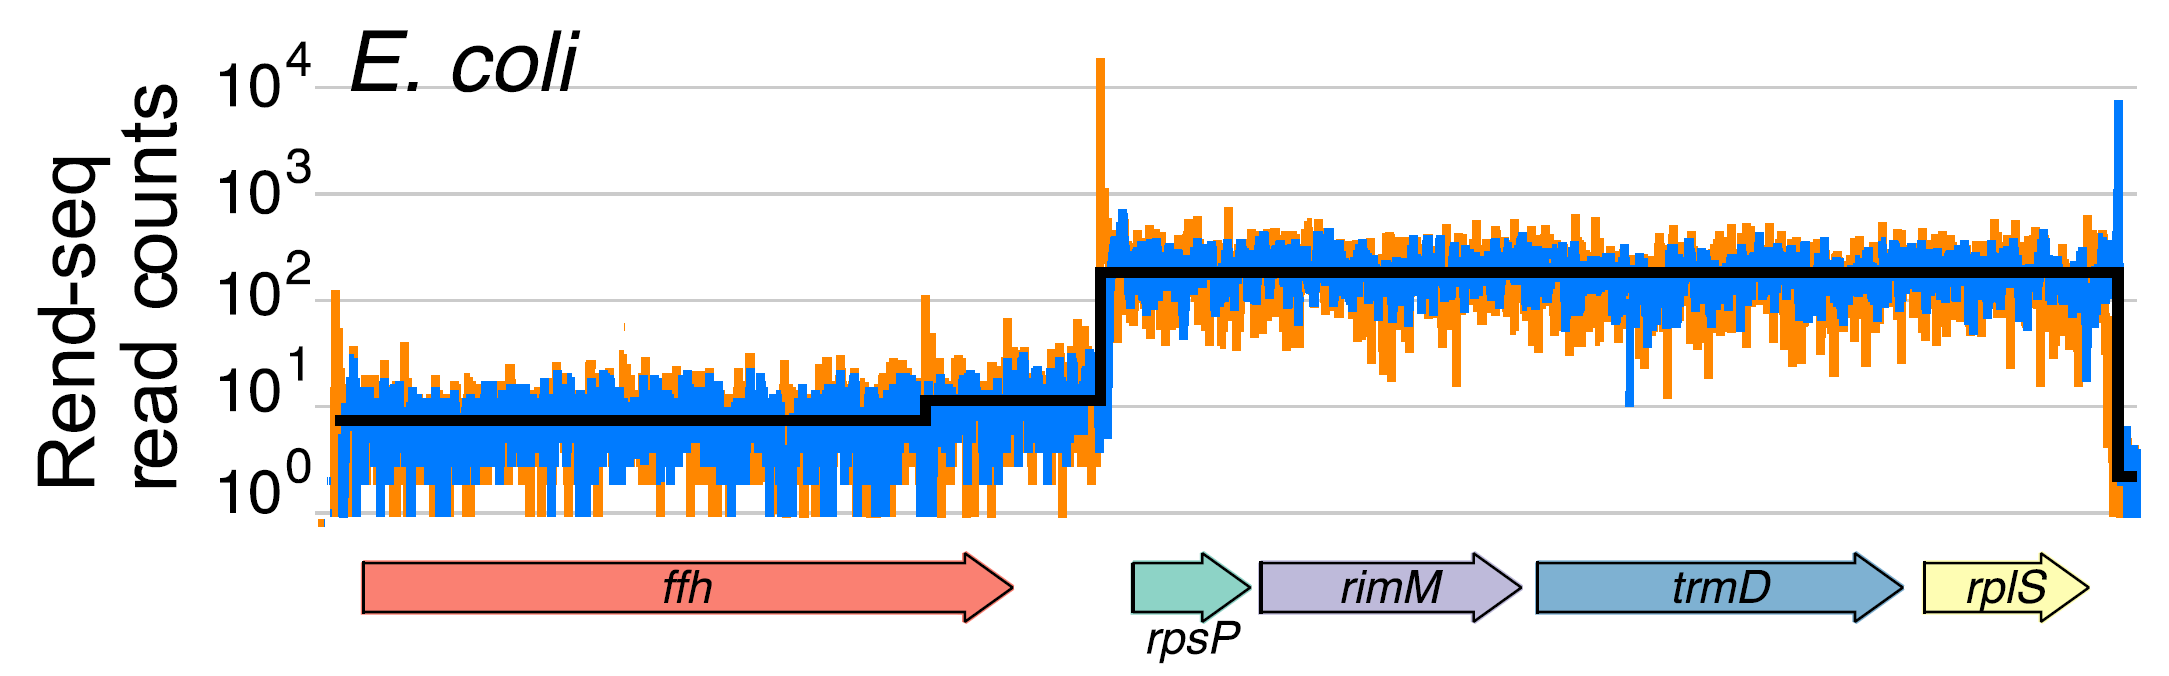
\includegraphics[width=0.6\textwidth]{lalanne_reads.png}
    \caption{Example data with genes. Orange and blue are reads, black indicates TUs.\textsuperscript{1}}
    \label{fig:lalanne_reads}
\end{figure}

\textbf{Method} \vspace{4pt} \\
For this work, I will be focusing on Rend seq data from \textit{E. coli} so the data input is $X\in \mathbb{R}^{9,279,350\text{x}2}$. The length of the genome is 4,639,675 base pairs with transcripts mapped to each genome location in both the forward and reverse direction for a total of 9,279,350 locations.  For each genome location, there are 2 values for reads, one in the 5' direction and one in the 3' direction.  Some processing of the data is required to better fit the algorithms.  The first thing that must be done is to segment the reads into regions separated by areas of no reads.  The goal is to determine the TU structure which will start and stop at certain places in the genome.  The algorithms used will handle small regions of genes better than analyzing the entire genome at once.  An example of this segmentation is shown below in Fig. \ref{fig:segmentation}:

\begin{figure}[H]
    \centering
    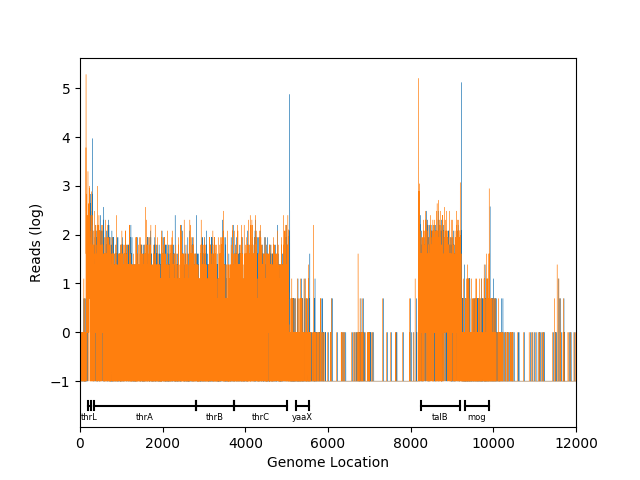
\includegraphics[align=c, width=0.25\textwidth]{both.png} $\boldsymbol{\longrightarrow}$
    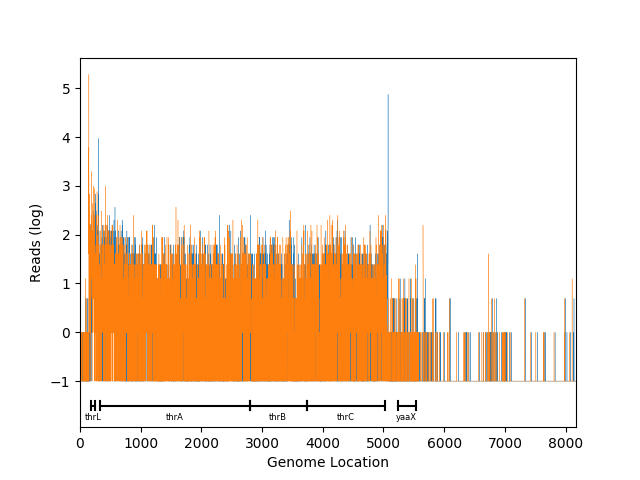
\includegraphics[align=c, width=0.25\textwidth]{0.png} $\boldsymbol{+}$
    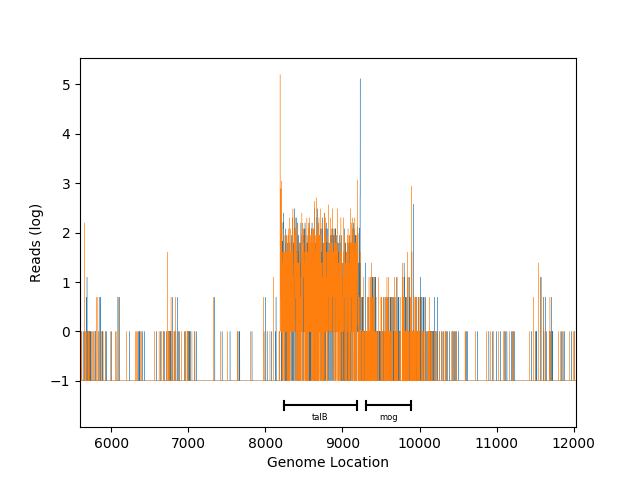
\includegraphics[align=c, width=0.25\textwidth]{1.png}
    \caption{Example of two read regions before (left of arrow) and after (right of arrow) segmentation.}
    \label{fig:segmentation}
\end{figure}

The data had to be further processed to transform the distribution to a Gaussian distribution to better fit the assumption made by the Gaussian mixture model and hidden Markov model.  Taking a moving average of the reads can transform the data from a Poisson distribution to a Gaussian distribution as illustrated in Fig. \ref{fig:distribution}.  This also has the added benefit of encoding some additional positional information into each point, which is useful because most neighboring positions will be in the same set of TUs.  Another possible transformation of the data is summing both the 3' and 5' reads and including a distance from the 3' and 5' reads at each location.  This will still have 2 features as before but more explicitly contain information about spikes in reads that will not be strand dependent (ie 3' spike vs 5' spike will appear the same).

\begin{figure}[H]
    \centering
    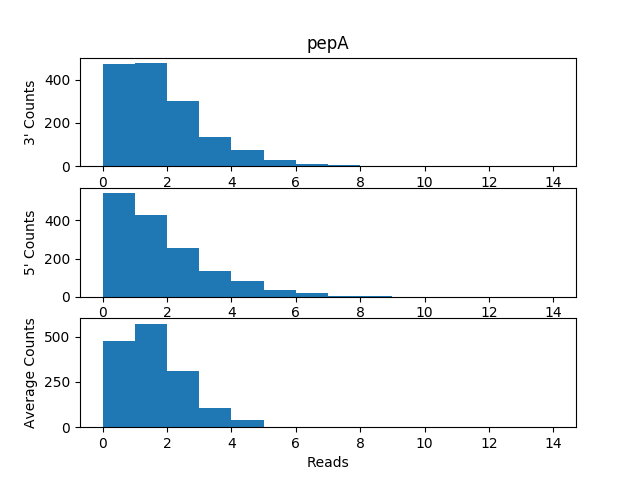
\includegraphics[width=0.3\textwidth]{pepA.png}
    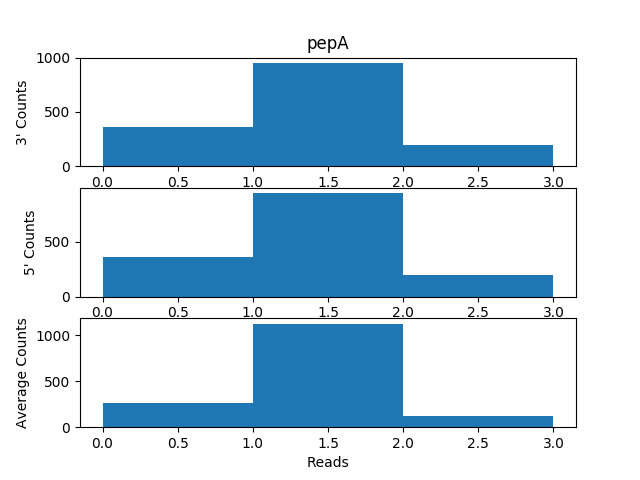
\includegraphics[width=0.3\textwidth]{pepA_ma.png}
    \caption{Transformation of read data for selected gene.  Single location read distribution (Poisson) is shown on the left and the distribution after taking a moving average (Gaussian) is on the right.}
    \label{fig:distribution}
\end{figure}

One of the first methods tried was applying a Gaussian mixture model (GMM) to determine the level of expression at different areas of the genome.  After applying a moving average, the distributions within each gene following a Gaussian distribution as shown in Fig. \ref{fig:distribution}.  The number of Gaussians for each region was variable based on the number of genes in the region plus three (additional Gaussian for blue spikes, orange spikes and areas where no transcription is expected).  Being able to determine the latent variable assignments would show the different TUs. \vspace{8pt}

A second method was a hidden Markov model (HMM).  Once again, this is a method that can provide insight into latent states of a system.  Each TU can be represented by the hidden states with the read counts being the signal that is emitted.  This algorithm more easily allows incorporation of physical knowledge about the system, potentially for better accuracy.  Since it is known that the start or end of a TU will correlate with a spike in the read counts on the 3' or 5' strand, the transition probabilities can be set up to capture this.  Specifically, there should be two hidden states for each TU, one short one for the transition and one long one for the length of the TU with transitions only able to progress from one TU to the next.  This means the transition probability matrix, $T$, will be built like the following, where $p_{gene}$ is the probability of seeing a gene (low) and $p_{transition}$ is the probability of leaving a transition (high):
\[T = \begin{bmatrix}
1-p_{gene} & p_{gene} & 0 & 0 & \dots & 0 \\
0 & 1-p_{transition} & p_{transition} & 0 & \dots & 0 \\
0 & 0 & 1-p_{gene} & p_{gene} & \dots & 0 \\
&& \vdots \\
0 & 0 & 0 & 0 & \dots & 1
\end{bmatrix}\]
% TODO: does this violate ergodicity of chain and is it required for HMM?

A third method incorporated was density-based spatial clustering of applications with noise (DBSCAN) clustering.  The spikes in read counts are outliers from the rest of the read data and signify the start or end of TUs.  Reliably identifying positions that contain spikes would solve the TU structure problem.  It would be expected that DBSCAN could identify these spikes as noise since they won't group with the majority of other locations that come from the same TU distribution. \\

\textbf{Preliminary experiments} \vspace{4pt} \\
I have explored the parameter space of the DBSCAN algorithm for several regions of genes.  This included varying the distance between points ($\epsilon$), minimum number of points in a cluster and the processing method of input data.  Although I do not have a numerical metric for the accuracy of this method, I have qualitatively compared it to what is expected for the identified regions and there is promising performance for some sets of parameters (see Fig. \ref{fig:results}). \vspace{8pt}

The input data for GMM and HMM have been varied to some extent to determine what works well for some regions.  This mostly includes looking at the moving average window size, input data type and the inclusion of surrounding data points.  Additionally, I have looked at the impact of different numbers of classes for both.  I have also tried an implementation for GMM where the weight in the E-step is determined by several locations around the desired location to capture sequence positional information.  Example raw output (read level of assigned latent state) of both methods is shown in Fig. \ref{fig:results}.  The example shown for HMM is the one with the highest score from several runs which had some large variability in assignments.

\begin{figure}[H]
    \centering
    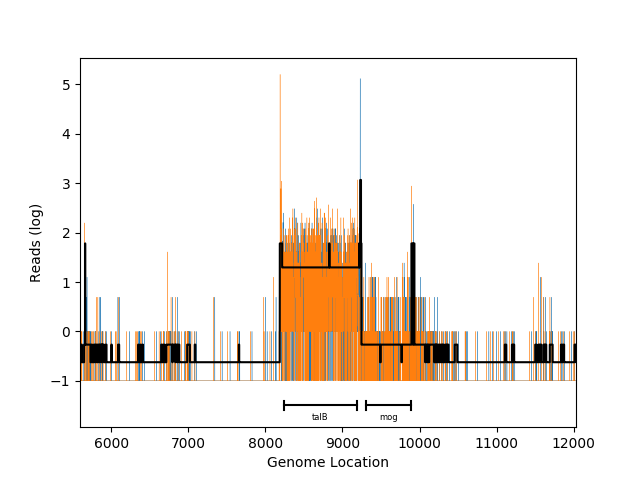
\includegraphics[align=c, width=0.25\textwidth]{1_gmm.png}
    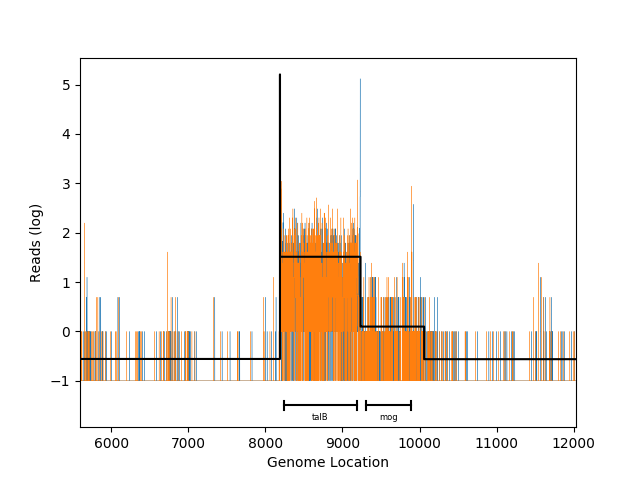
\includegraphics[align=c, width=0.25\textwidth]{1_hmm.png}
    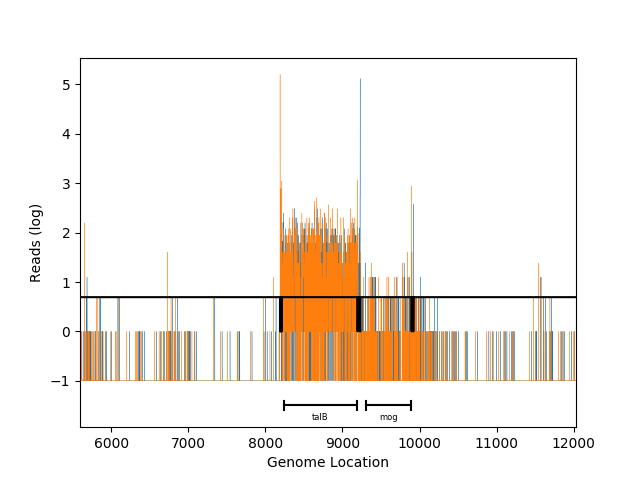
\includegraphics[align=c, width=0.25\textwidth]{1_dbscan.png}
    \caption{Black traces show results from the three methods (GMM, HMM, DBSCAN) for one region.}
    \label{fig:results}
\end{figure}

% Results for region 1
% GMM: window=15, total, n_levels=genes+3, modifiedGaussian
% HMM: window=1, total, n_levels=2*genes+2
% DBSCAN: window=1, total, eps=3, min_samples=5
\textbf{Next steps} \vspace{4pt} \\
A major next step will be to convert the output from each algorithm into a concrete prediction of TU start and end positions.  Once this is done, I will be able to create a performance metric to more easily compare outcomes from specific parameter changes.  I plan to annotate a subset of gene regions to use as a validation set while the rest of the genome can remain a qualitative test set without annotations.  The HMM and DBSCAN methods should produce output with discrete signals that can easily be converted, however, the GMM output may need further processing since many times the output will alternate between classifications for nearby sequence locations.  I expect feeding the probabilities for each class at each genome location into a HMM would be able to maximize the expectation subject to the physical constraints of TU structure. \vspace{8pt}

With a proper metric, I will be able to perform a larger parameter sweep for each method.  For all methods, the processing of input data (moving average window size, summed reads, data from neighboring points, other methods to encode genome position information) will be a major parameter.  For GMM and HMM, the number of possible latent states can also be explored.  It might also be useful to implement both methods based on a Poisson data distribution instead of Gaussian. \vspace{8pt}

Finally, a few more general ideas.  I plan to refine the region segmentation to get more precise regions which do not contain extraneous reads unrelated to any gene TUs. I would also like to think about better ways to incorporate read spikes as high probability for transitions. \\

\textbf{\footnotesize References} \vspace{1pt} \\
{\footnotesize
1. Lalanne JB, \textit{et al.} (2018). Evolutionary Convergence of Pathway-Specific Enzyme Expression Stoichiometry. \textit{Cell} 173(3) 749-761. \\
2. Karr, JR, \textit{et al.} (2012). A whole-cell computational model predicts phenotype from genotype. \textit{Cell} 150(2) 389-401.
}
\end{document}